\documentclass[11pt, a4paper]{article}
\PassOptionsToPackage{hidelinks}{hyperref} 
\usepackage[utf8]{inputenc} 
\usepackage{fullpage}
\usepackage{graphicx}
\usepackage{xcolor}
\usepackage{amsmath}
\usepackage{bookmark}
\usepackage{ragged2e}
\usepackage{amsmath}
\usepackage{amsfonts}
\usepackage{array}
\usepackage{float}
\usepackage{tabularx}
\usepackage{listings}
\usepackage{hyperref}
\usepackage[backend=biber]{biblatex}
\renewcommand\UrlFont{\color{blue}\rmfamily}
 
% Title of your project
\title{Prediction with Back-Propagation and Linear Regression }

% Name of deliverable
\newcommand{\deliverableName}{Delivery of Activity 1}

% Author
\author{Javier Novella Ruiz}

% Group number
\newcommand{\groupNumber}{17685106}

% Comment
\newcommand{\comments}{Virtual student}

% Date for title page, default is today and 
\date{\today}

\makeatletter{}

\setlength{\parindent}{0pt}

\begin{document}

\begin{titlepage}
  	\newcommand{\HRule}{\rule{\linewidth}{0.3mm}}
	\center
	%------------------------------------------------
	%	Headings
	%------------------------------------------------
	
	\textsc{\LARGE Universitat Rovira i Virgili}\\[1.5cm]
	
	\textsc{\Large \deliverableName}\\[0.5cm]
	
	\textsc{\large Neural and Evolutionary Computation}\\[0.5cm]
	
	%------------------------------------------------
	%	Title
	%------------------------------------------------
	
	\HRule\\[0.4cm]
	
	{\huge\bfseries \@title}\\[0.4cm]
	
	\HRule\\[1.5cm]
	
	%------------------------------------------------
	%	Author(s)
	%------------------------------------------------

 	{\large\sc\@author}
	
	%------------------------------------------------
	%	Date
	%------------------------------------------------
	
	\vfill\vfill
	%	{\large\@date}
    \vfill\vfill\vfill
	
	%------------------------------------------------
	%	Logo
	%------------------------------------------------
	\vfill
	
\includegraphics[width=0.3\textwidth]{./urvlogo.png}
	\vfill
\end{titlepage}


\tableofcontents

\newpage

\section{Introduction}

The goal of this activity is to practice with different types of supervised models. In particular, the following methods have been used. 
\begin{itemize}
    \item Neural Network with Back-Propagation BP, implemented by the author of this report.
    \item Neural Network with Back-Propagation BP-F, using keras library.
    \item Multiple Linear Regression MLR-F, using the sklearn python library.
\end{itemize}

To achieve this purpose firstly the a dataset has been selected, analyzed and pre-processed. Then the methods commented before have been
applied to the dataset to obtain predictions of values.

\subsection{GitHub repository}

The Jupyter Notebook and the module with the BP devolpemnt together with the dataset files and image results can be consulted in
the following GitHub repository (\href{https://github.com/novella93/NEC_A1}{Link to Javier Novella NEC A1 repository}).

\vspace{1em} From the descriptions and explanations point of view, the Jupyter Notebook file A1.ipynb contains a retailed version of this 
report in the markdowns. But it contains all the Python code used to obtain the results for this report.

\vspace{1em} For the BP implementation the file BP.py is the module which implements the NeuralNet Class, and can be found also in the same
repository.

\newpage

\section{Dataset}

The dataset used include data for the estimation of obesity levels in individuals from the countries of Mexico, Peru and Colombia, based 
on their eating habits and physical condition. The data contains 17 attributes and 2111 records. The dataset source is UCI Machine Learning 
Repository \href{https://archive.ics.uci.edu/dataset/544/estimation+of+obesity+levels+based+on+eating+habits+and+physical+condition}{(Link to the dataset repository)}.

\vspace{1em} Note: all the results and calculations obtained in this chapter can be found in the file A1.ipynb in the GitHub repository 
(\href{https://github.com/novella93/NEC_A1/blob/main/A1.ipynb}{Link to A1.ipynb in Javier Novella NEC A1 repository})

\vspace{1em} The dataset is composed by the following features:

\begin{itemize}
    \item \textbf{Gender}: gender of the individual.
    \item \textbf{Age}: age of the individual.
    \item \textbf{Height}: height of the individual.
    \item \textbf{Weight}: weight of the individual.
    \item \textbf{family\_history\_with\_overweight}: Has a family member suffered or suffers from overweight?
    \item \textbf{FAVC}: Does the individual eat high caloric food frequently?
    \item \textbf{FCVC}: Does the individual usually eat vegetables in your meals?
    \item \textbf{NCP}: How many main meals does the individual have daily?
    \item \textbf{CAEC}: Does the individual eat any food between meals?
    \item \textbf{SMOKE}: Does the individual smoke?
    \item \textbf{CH20}: How much water does the individual drink daily?
    \item \textbf{SCC}: Does the individual monitor the calories eaten daily?
    \item \textbf{FAF}: How often the individual has physical activity?
    \item \textbf{TUE}: How much time does the individual use technological devices such as cell phone, videogames, television, computer and others?
    \item \textbf{CALC}: How often does the individual drink alcohol?
    \item \textbf{MTRANS}: Which transportation does the individual usually use?
    \item \textbf{NObeyesdad}: Obesity level
\end{itemize}

\newpage

\subsection{Inputs and output selection}

From the 17 features, 16 of them are considered inputs and 1 is considered output.

\begin{itemize}
    \item \textbf{Inputs:}
    \begin{itemize}
        \item Gender
        \item Age
        \item Height
        \item Weight
        \item family\_history\_with\_overweight
        \item FAVC
        \item FCVC
        \item NCP
        \item CAEC
        \item SMOKE
        \item CH20
        \item SCC
        \item FAF
        \item TUE
        \item CALC
        \item MTRANS
    \end{itemize}
    \item \textbf{Outputs:}
    \begin{itemize}
        \item NObeyesdad
    \end{itemize}
\end{itemize}

\subsection{Output transformation}

The output NObeyesdad allows classification of the data using the values of Insufficient Weight, Normal Weight, Overweight Level I, 
Overweight Level II, Obesity Type I, Obesity Type II and Obesity Type III. As the predicted variable must be a real value \(float or double\) 
this value will be replaced by the corresponding \(BMI\).

\vspace{1em}The Body Mass Index \(BMI\) is a simple calculation using a person's height and weight. The formula is \(BMI = \frac{weight}{height^{2}}\) 
\((\frac{kg}{m^{2}})\). It is used as an indicator of whether an individual is underweight, normal weight, overweight, or obese. The correspondance from the 
previous  categorical values to the new numerical ones are:

\begin{itemize}
    \item \textbf{Insufficient Weight (Underweight)}: BMI less than 18.5
    \item \textbf{Normal Weight}: BMI between 18.5 and 24.9
    \item \textbf{Overweight Level I (Pre-obesity)}: BMI between 25 and 29.9
    \item \textbf{Overweight Level II}: BMI between 30 and 34.9
    \item \textbf{Obesity Type I}: BMI between 35 and 39.9
    \item \textbf{Obesity Type II}: BMI between 40 and 44.9
    \item \textbf{Obesity Type III}: BMI 45 and above
\end{itemize}

To achive this result, the value of the column "NObeyesdad" is replaced by the mentioned formula \(BMI = \frac{weight}{height^{2}}\) using 
the weight and height within the same record processed. This will result in the \(BMI\) calcualted for each individual which is a real numeric value.

\subsection{Dataset checks}

The data will be checked for the following points:

\begin{itemize}
    \item Check for missing values
    \item Check for duplicates
    \item Check data type
    \item Check unique values on each column
\end{itemize}

\subsubsection{Check missing values}

The dataset is fully checked for null values feature by feature. No missing values are found in during this search.

\begin{table}[H]
    \centering
    \begin{tabular}{|c|c|c|}
        \hline
        \textbf{Feature} & \textbf{Number of missing values} \\ \hline
        Gender & 0 \\ \hline
        Age & 0 \\ \hline
        Height & 0 \\ \hline
        Weight & 0 \\ \hline
        family\_history\_with\_overweight & 0 \\ \hline
        FAVC & 0 \\ \hline
        FCVC & 0 \\ \hline
        NCP & 0 \\ \hline
        CAEC & 0 \\ \hline
        SMOKE & 0 \\ \hline
        CH2O & 0 \\ \hline
        SCC & 0 \\ \hline
        FAF & 0 \\ \hline
        TUE & 0 \\ \hline
        CALC & 0 \\ \hline
        MTRANS & 0 \\ \hline
        Nobeyesdad & 0 \\ \hline
    \end{tabular}
    \caption{Number of missing values within the full dataset}
    \label{tab:table_missing_values}
\end{table}

\subsubsection{Check duplicates}

24 records are duplicated. This means that the dataset contains information about 24 individuals that have exactly the same features. 
In this case, this duplicates are kept because it is assumed that they represent legitimate repeated records from different people.

\subsubsection{Check datatypes}

Check data types allows to make a first sight to know which features are numerical and which are categorical. This will help in the further 
pre-processing steps to know which fields must be transformed/normalized. In this case the features are:

\begin{table}[H]
    \centering
    \begin{tabular}{|c|c|c|}
        \hline
        \textbf{Feature} & \textbf{Data type} & \textbf{Type} \\ \hline
        Gender & object & Categorical \\ \hline
        Age & float64 & Numerical \\ \hline
        Height & float64 & Numerical \\ \hline
        Weight & float64 & Numerical \\ \hline
        family\_history\_with\_overweight & object & Categorical \\ \hline
        FAVC & object & Categorical \\ \hline
        FCVC & float64 & Numerical \\ \hline
        NCP & float64 & Numerical \\ \hline
        CAEC & object & Categorical \\ \hline
        SMOKE & object & Categorical \\ \hline
        CH2O & float64 & Numerical \\ \hline
        SCC & object & Categorical \\ \hline
        FAF & float64 & Numerical \\ \hline
        TUE & float64 & Numerical \\ \hline
        CALC & object & Categorical \\ \hline
        MTRANS & object & Categorical \\ \hline
        NObeyesdad & float64 & Numerical \\ \hline
    \end{tabular}
    \caption{Data types of each feature}
    \label{tab:table_data_types}
\end{table}

\subsubsection{Check unique values by feature}

Understanding the range of unique values in categorical variables will help in choosing the right encoding techniques.

\begin{table}[H]
    \centering
    \begin{tabular}{|c|c|c|}
        \hline
        \textbf{Feature} & \textbf{Number of unqiue values} \\ \hline
        Gender & 2 \\ \hline
        Age & 1402 \\ \hline
        Height & 1574 \\ \hline
        Weight & 1525 \\ \hline
        family\_history\_with\_overweight & 2 \\ \hline
        FAVC & 2 \\ \hline
        FCVC & 810 \\ \hline
        NCP & 635 \\ \hline
        CAEC & 4 \\ \hline
        SMOKE & 2 \\ \hline
        CH2O & 1268 \\ \hline
        SCC & 2 \\ \hline
        FAF & 1190 \\ \hline
        TUE & 1129 \\ \hline
        CALC & 4 \\ \hline
        MTRANS & 5 \\ \hline
        Nobeyesdad & 1340 \\ \hline
    \end{tabular}
    \caption{Number of unique values by feature}
    \label{tab:table_unique_values}
\end{table}

\subsection{Statistics}

The dataset consists of 2111 records and 17 features, with each record considered unique despite some duplications. 
Importantly, there are no null values in the dataset, ensuring completeness. The features cover aspects of individuals' health and lifestyle, 
including height, weight, vegetable intake, number of main meals, water consumption, sports activity, use of technological devices, and BMI.

\begin{table}[H]
    \centering
    \begin{tabular}{|c|c|c|c|c|c|c|c|c|c|}
        \hline
              &    Age   & Height   & Weight   & FCVC     & NCP      & CH2O     & FAF      & TUE        & NObeyesdad \\ \hline 
        count &     2111 & 2111     & 2111     & 2111      & 2111    & 2111     & 2111     & 2111       & 2111 \\ \hline
        mean  & 24.310   & 1.700    & 86.590   & 2.420    & 2.690    & 2.010    & 1.010    & 0.660      & 29.700   \\ \hline
        std   & 6.350    & 0.090    & 26.190   & 0.530    & 0.780    & 0.610    & 0.850    & 0.610      & 8.010    \\ \hline
        min   & 14.000   & 1.450    & 39.000   & 1.000    & 1.000    & 1.000    & 0.000    & 0.000      & 13.000   \\ \hline
        25\%  & 19.950   & 1.630    & 65.470   & 2.000    & 2.660    & 1.580    & 0.120    & 0.000      & 24.330   \\ \hline
        50\%  & 22.780   & 1.700    & 83.000   & 2.390    & 3.000    & 2.000    & 1.000    & 0.630      & 28.720   \\ \hline
        75\%  & 26.000   & 1.770    & 107.430  & 3.000    & 3.000    & 2.480    & 1.670    & 1.000      & 36.020   \\ \hline
        max   & 61.000   & 1.980    & 173.000  & 3.000    & 4.000    & 3.000    & 3.000    & 2.000      & 50.810   \\ \hline
    \end{tabular}
    \caption{Statistics from the dataset}
    \label{tab:table_statistics}
\end{table}

\vspace{1em}The dataset shows a range of values for these features. Heights range from 1.45 to 1.98 meters, and weights range from 39.0 to 173.0 kilograms. 
Individuals consume between 1 to 3 pieces of vegetables per day and have 1 to 4 main meals daily. Water intake varies from 1 to 3 liters per day, 
sports activity ranges from 0 to 3 hours per day, and use of technological devices ranges from 0 to 2 hours per day. BMI values span 
from 13.0 to 50.81 kg/m², indicating a wide range of body compositions.

\vspace{1em}In terms of data distribution, the features with the highest variability are age, weight, and obesity level. The averages of these features are 
close to the 50th percentile, suggesting that the data is evenly distributed. This balanced distribution is beneficial for analysis, as it 
indicates that the dataset provides a comprehensive representation of the population's health and lifestyle characteristics.

\subsubsection{Categorical features}

The categorical features and its exposed in the Table \ref{tab:table_categorical_values}.

\begin{table}[H]
    \centering
    \begin{tabular}{|c|c|}
        \hline
        \textbf{Feature} & \textbf{Possible values} \\ \hline
        Gender & ['Female' 'Male'] \\ \hline
        family\_history\_with\_overweight & ['yes' 'no'] \\ \hline
        FAVC & ['no' 'yes'] \\ \hline
        CAEC & ['Sometimes' 'Frequently' 'Always' 'no'] \\ \hline
        SMOKE & ['no' 'yes'] \\ \hline
        SCC & ['no' 'yes'] \\ \hline
        CALC & ['no' 'Sometimes' 'Frequently' 'Always'] \\ \hline
        MTRANS & ['Public\_Transportation' 'Walking' 'Automobile', \\
               & 'Motorbike' 'Bike'] \\ \hline
    \end{tabular}
    \caption{Possible values of the categorical features}
    \label{tab:table_categorical_values}
\end{table}

In the Figure \ref{fig:image_distribution_categorical_features} it shown the distribution of the categorical data. Showing the distribution 
is important when analyzing a dataset for neural network usage because it helps identify imbalances and patterns within the data. This understanding 
can help training on a representative sample, and this can improve its accuracy and generalization. It also shows any potential biases, allowing for 
adjustments to be made to achieve good predictions.

\begin{figure}[H]
    \centering
    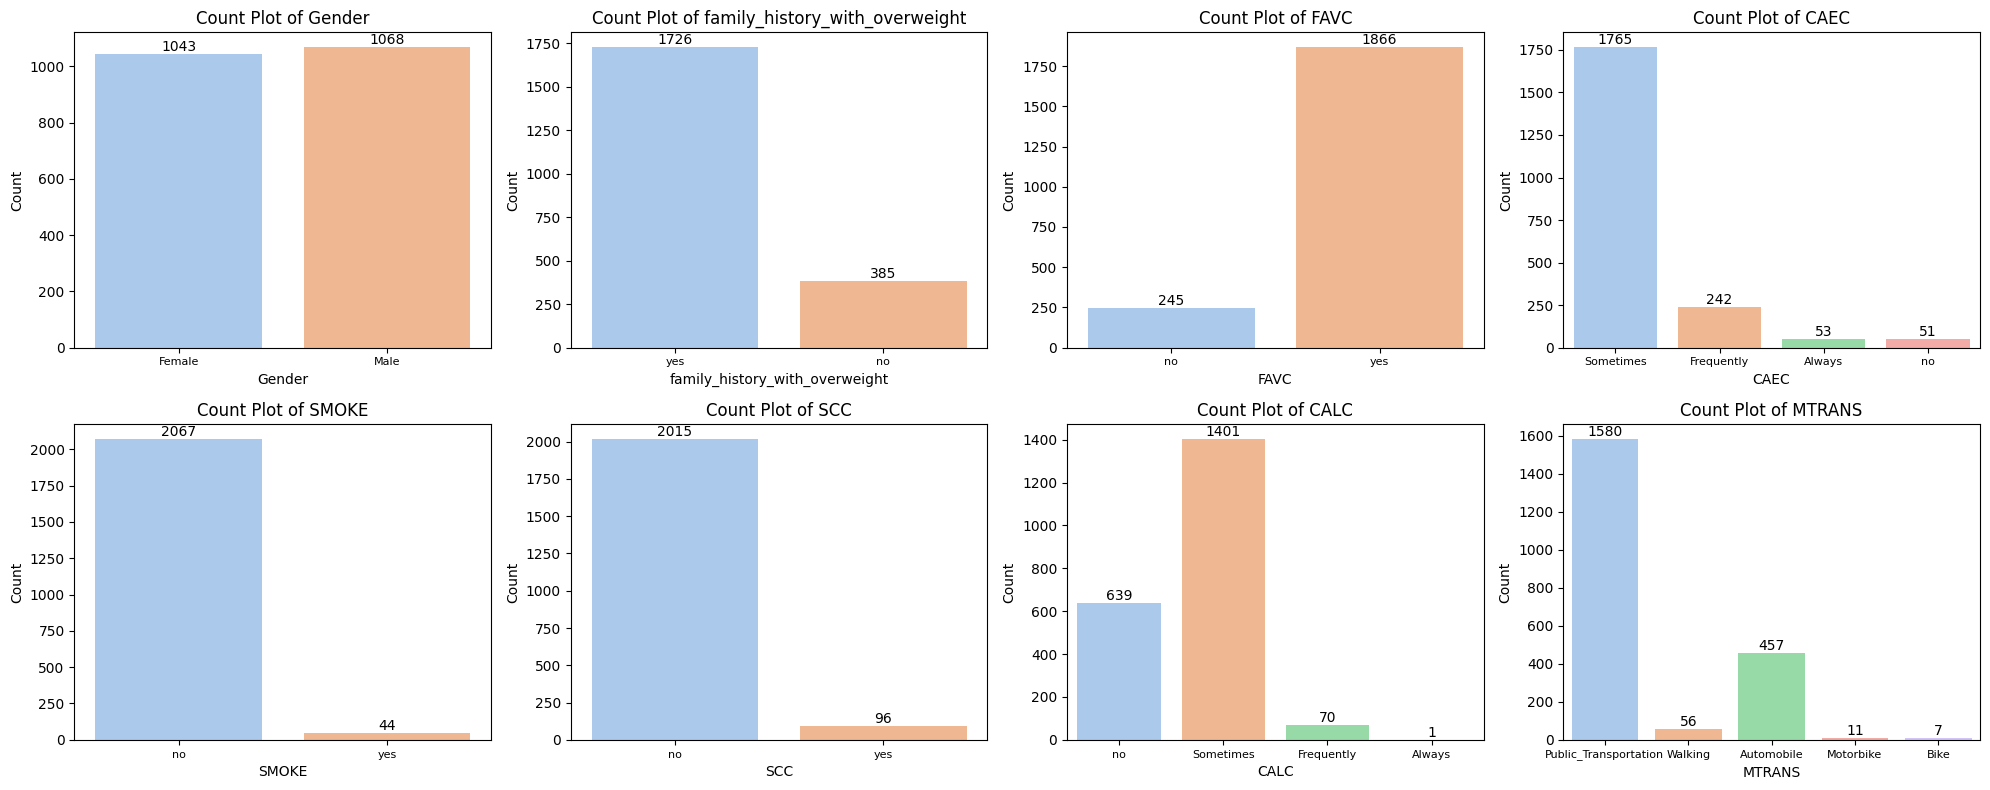
\includegraphics[width=\textwidth]{images/distribution_categorical_features.png}
    \caption{Distribution of the categorical features}
    \label{fig:image_distribution_categorical_features}
\end{figure}

But the get more insights it is interesting to get the boxplot of the categorical features against the output feature that is the obesity level.
This is shown in the Figure \ref{fig:image_categorical_features_vs_obesity_level}. This view provide a clear summary of the distribution, 
central tendency, and variability of obesity levels within each category. This helps identify patterns, outliers, and differences between groups, 
making it easier to understand how different categorical factors influence obesity.

\begin{figure}[H]
    \centering
    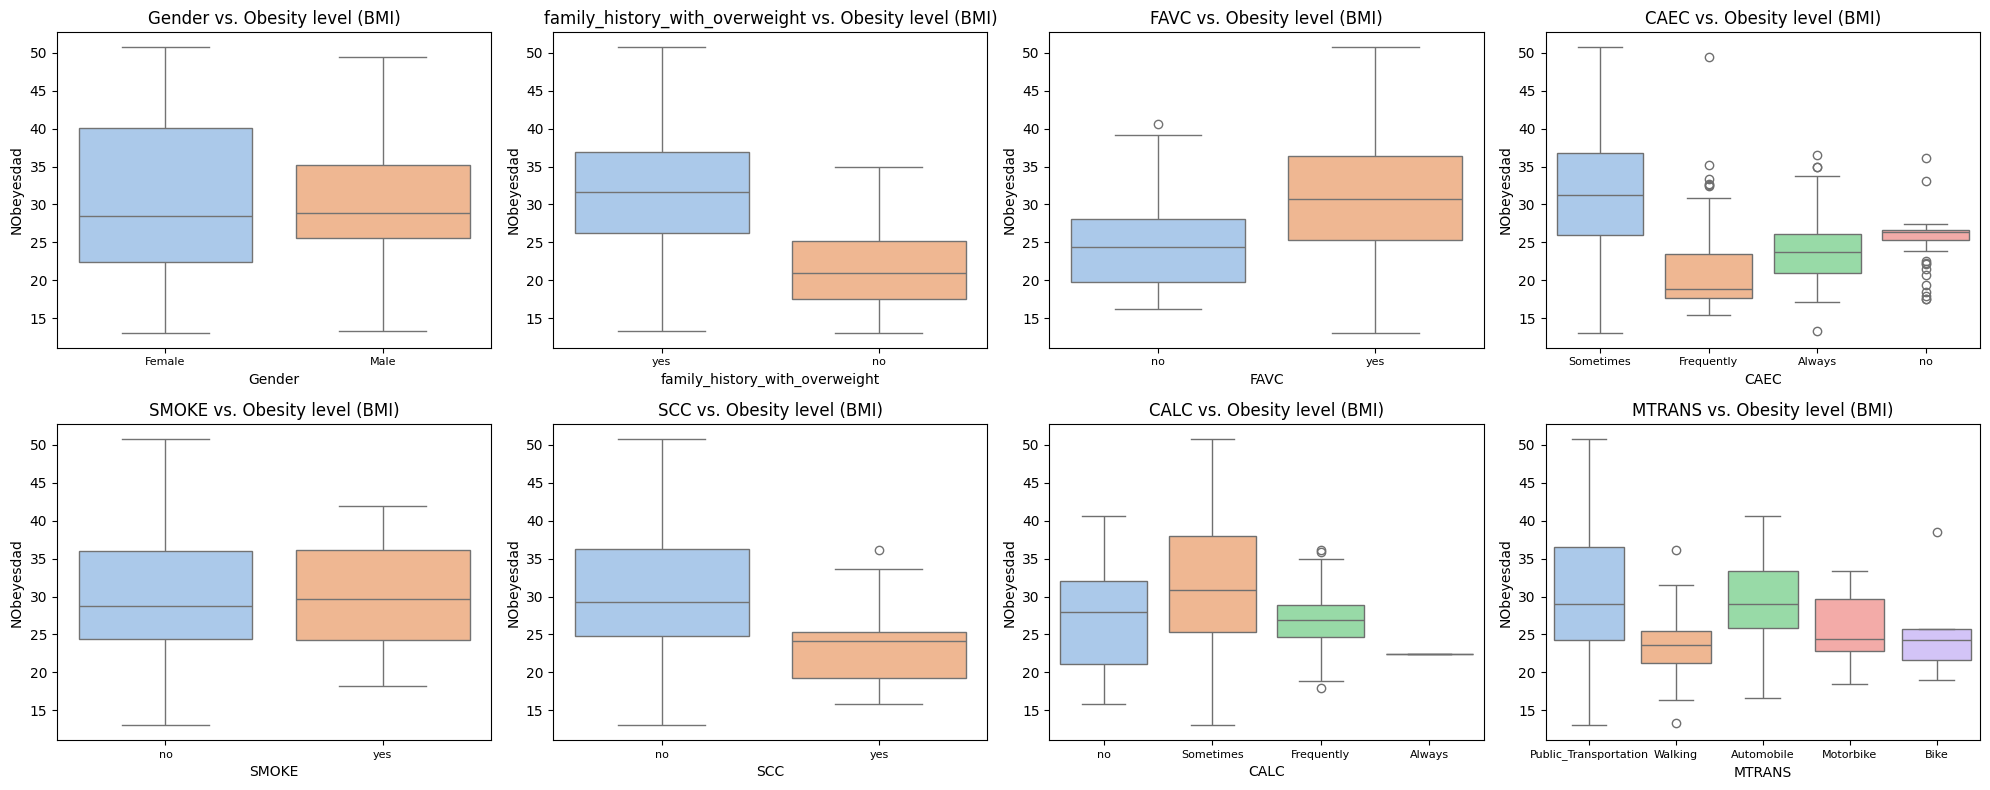
\includegraphics[width=\textwidth]{images/categorical_features_vs_obesity_level.png}
    \caption{Categorical features vs obesity level}
    \label{fig:image_categorical_features_vs_obesity_level}
\end{figure}

From this data, can be exposed that males tend to have higher levels of obesity compared to females. High caloric diets are associated with increased 
obesity levels, while controlling calorie intake helps in maintaining lower obesity levels. Interestingly, smoking does not seem to impact obesity levels 
significantly.

\vspace{1em}Additionally, individuals who use active transportation methods like walking or biking tend to have lower obesity levels. These findings 
highlight the importance of diet and physical activity in managing obesity.

\subsubsection{Numerical features}

In the Figure \ref{fig:image_distribution_numerical_features} it shown the distribution of the numerical data. Showing the distribution of numerical 
features using histograms is important because it helps visualize the data's shape, central tendency, and spread.

\begin{figure}[H]
    \centering
    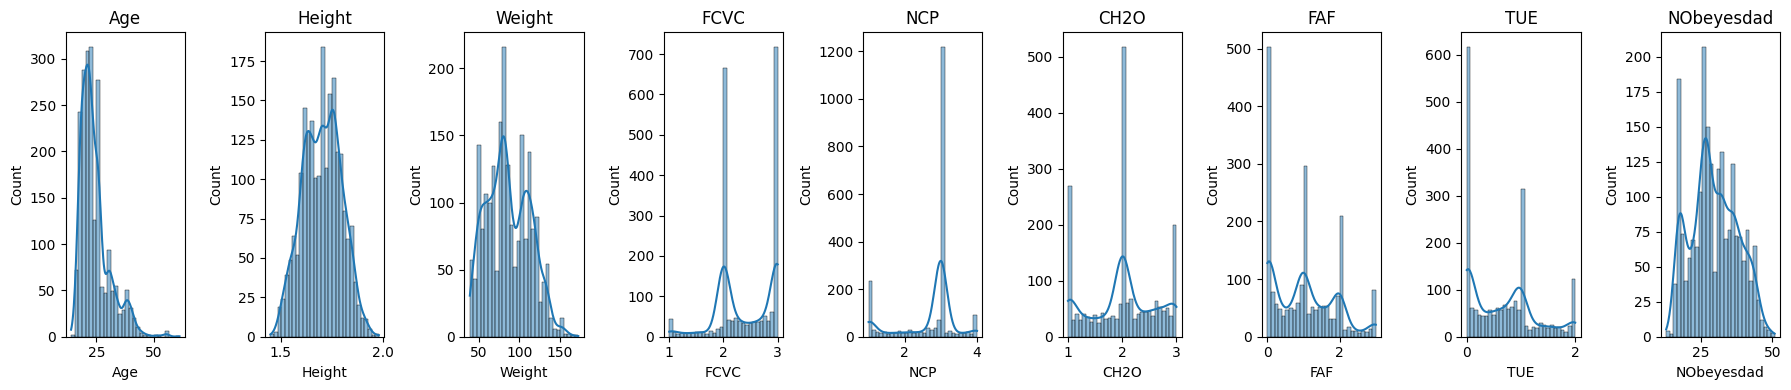
\includegraphics[width=\textwidth]{images/distribution_numerical_features.png}
    \caption{Distribution of the numerical features}
    \label{fig:image_distribution_numerical_features}
\end{figure}

It is interesting to focus on the output variable, to get more insights from the dataset, this is shown in the Figure \ref{fig:image_distribution_obesity_level}.
Focusing on the distribution of the obesity level, is crucial because it helps understand the range and variability of the variable. 

\begin{figure}[H]
    \centering
    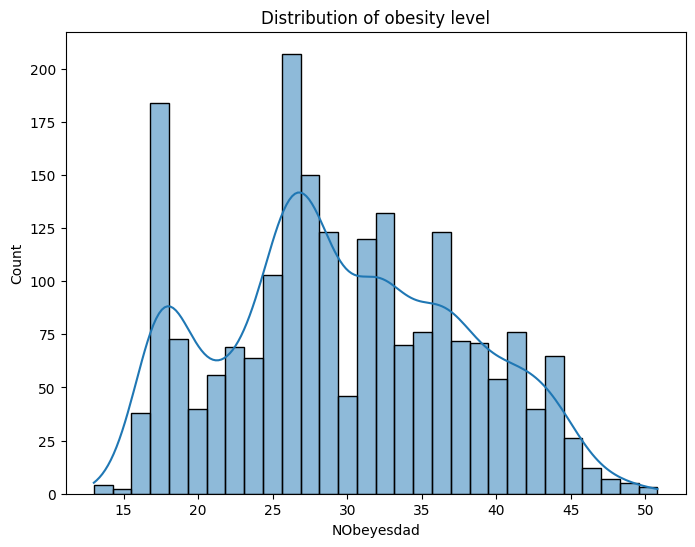
\includegraphics[width=300pt]{images/distribution_obesity_level.png}
    \caption{Distribution of the obesity level}
    \label{fig:image_distribution_obesity_level}
\end{figure}

The relation between this numerical data and its affectance to the output variable can be seen in the correlation matrix shown in the 
Figure \ref{fig:image_correlation_matrix_between_features}. A heatmap of the correlation matrix is used because it visually represents 
the strength and direction of relationships between the numerical features. This helps identify which features are strongly correlated 
with each other and also with the obesity level.

\begin{figure}[H]
    \centering
    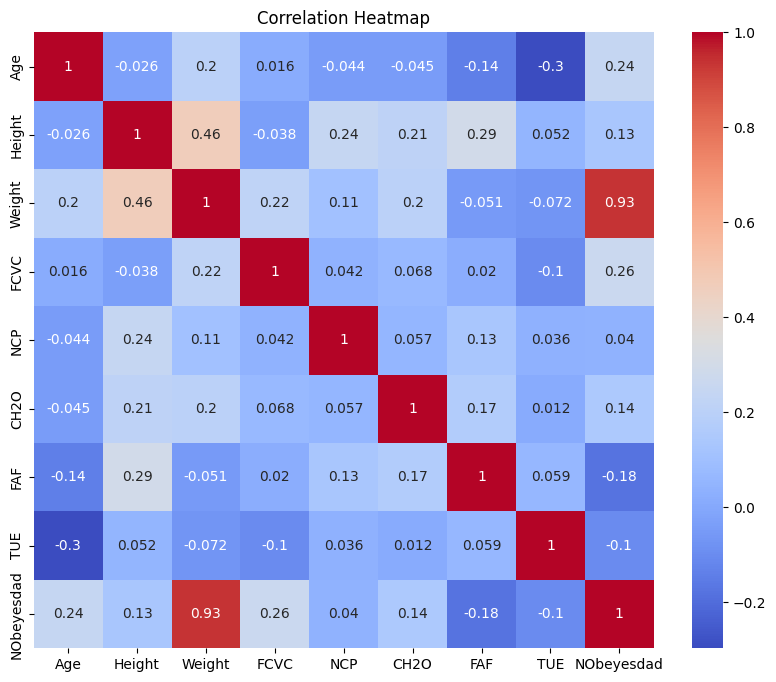
\includegraphics[width=300pt]{images/correlation_matrix_between_features.png}
    \caption{Coorrelation matrix between numerical features}
    \label{fig:image_correlation_matrix_between_features}
\end{figure}

From this data is deduced taht the individuals in the dataset have a BMI ranging from 13.0 to 50.81 kg/m². The average obesity level is 29.7, 
which corresponds to Overweight Level I, close to the threshold for Overweight Level II. It is important to note that there is high variability 
in obesity levels, with 25\% of individuals having normal BMI values \((BMI < 25)\).

Moreover the features with the highest impact on obesity levels, in decreasing order, are Weight, FCVC: frequency of consumption of vegetables, 
Age, CH20: water consumption, and Height.

\subsection{Data preprocessing}

The data is splitted in two different datasets, the training and test datasets. The training dataset contains the 16 input features stated before 
while the test data set only contains the output fetaure NObeyesdad=Obesity level. The datasets are created from the main dataset with 2111 records 
and it is splitted such 80\% of the records (1688) are in the train set and the 20\% remaining (423) are in the test set. From this train set the 
75\% of the records is kept as training set (1583) and the 25\% of the records (528) is used as validation data.

\vspace{1em}The following categorical features has been adjusted for integer values, this is suitable because the categorical features in the dataset have an 
inherent order (low, medium, high etc.) or the features are binary which can be converted from the 2 binary values to 0 and 1, which is a 
straightforward and effective change.

\begin{table}[H]
    \centering
    \begin{tabular}{|c|c|}
        \hline
        \textbf{Feature} & \textbf{Type} \\ \hline
        Gender &  Categorical \\ \hline
        family\_history\_with\_overweight & Categorical \\ \hline
        FAVC &  Categorical \\ \hline
        CAEC &  Categorical \\ \hline
        SMOKE &  Categorical \\ \hline
        SCC &  Categorical \\ \hline
        CALC &  Categorical \\ \hline
        MTRANS &  Categorical \\ \hline
    \end{tabular}
    \caption{Categorical features preprocessed}
    \label{tab:table_categorical_preprocessing}
\end{table}

The following numerical values has been normalized. This is important to improve convergence speed and accuracy, preventing feature dominance and 
improving interpretability.

\begin{table}[H]
    \centering
    \begin{tabular}{|c|c|}
        \hline
        \textbf{Feature} & \textbf{Type} \\ \hline
        Age &  Numerical \\ \hline
        Height &  Numerical \\ \hline
        Weight &  Numerical \\ \hline
        FCVC &  Numerical \\ \hline
        NCP &  Numerical \\ \hline
        CH2O &  Numerical \\ \hline
        FAF &  Numerical \\ \hline
        TUE &  Numerical \\ \hline
        NObeyesdad &  Numerical \\ \hline
    \end{tabular}
    \caption{Numerical features preprocessed}
    \label{tab:table_numerical_preprocessing}
\end{table}

\section{Implementation of BP}

The BP Python module includes activation functions and the NeuralNet class for implementing neural networks with backpropagation. The module provides 
several activation functions: Sigmoid, ReLU, Leaky ReLU, Tanh, and Linear.  It has attributes like network structure, epochs, learning rate, and momentum. 
The activation function can be selected using the fact parameter.

\vspace{1em} Note: this implementation can be found in the file BP.py in the GitHub repository 
(\href{https://github.com/novella93/NEC_A1/blob/main/BP.py}{Link to BP.py in Javier Novella NEC A1 repository})

\subsection{NeuralNet class}

\subsubsection{Attributes}

The list of attributes and their descriptions are the following ones:

\begin{itemize}
    \item \textbf{Network Structure}: The layers attribute specifies the number of neurons in each layer.
    \item \textbf{Epochs}: The epochs attribute defines the number of training iterations.
    \item \textbf{Learning Rate}: The learning\_rate attribute controls the step size during gradient descent.
    \item \textbf{Momentum}: The momentum attribute helps accelerate gradients vectors in the right directions.
    \item \textbf{Activation Function}: The fact attribute allows selecting the activation function to be used in the network.
\end{itemize}

\subsubsection{Private methods}

The \textbf{\_select\_activation\_function()} method dynamically selects the appropriate activation function based on the fact parameter. It supports functions like 
sigmoid, relu, leaky relu, tanh, and linear.

\vspace{1em}The \textbf{\_select\_derivative\_activation\_function()} method selects the derivative of the activation function, which is for backpropagation. 
It matches the activation function chosen by \_select\_activation\_function().

\vspace{1em}The \textbf{\_forward\_propagation()} method passes input data through the network layer by layer. It applies weights, thresholds, and activation functions 
to compute the output of each layer.

\vspace{1em}The \textbf{\_backward\_propagation()} method calculates the output error and propagates it backward through the network. It updates weights and thresholds 
using gradient descent with momentum to minimize the error.

\vspace{1em}The \textbf{\_train()} method normalizes input data and trains the network using mini-batch gradient descent. It periodically computes the training and 
validation loss to monitor the network's performance.

\subsubsection{Public methods}

The \textbf{fit()} method normalizes input data and trains the network. It calls the \_train() method to perform the training process.

\vspace{1em}The \textbf{predict()} method normalizes input data and performs a forward pass through the network to generate predictions on new data.

\vspace{1em}The \textbf{loss\_epochs()} method returns the training and validation loss for each epoch.

\subsection{Activation functions}

\subsubsection{Sigmoid}

The sigmoid activation function is defined as:

$$ \sigma(x) = \frac{1}{1 + e^{-x}} $$

Its derivative is:

$$ \sigma'(x) = \sigma(x) \cdot (1 - \sigma(x)) $$

\subsubsection{ReLU}

On the one hand, the ReLU (Rectified Linear Unit) activation function is defined as:

$$ \text{ReLU}(x) = \max(0, x) $$

Its derivative is:

$$
\text{ReLU}'(x) = \begin{cases} 
1 & \text{if } x > 0 \\ 
0 & \text{if } x \leq 0 
\end{cases}
$$

On the other, the Leaky ReLU activation function is defined as:

$$
\text{Leaky ReLU}(x) = \begin{cases} 
x & \text{if } x > 0 \\ 
\alpha x & \text{if } x \leq 0 
\end{cases}
$$

Its derivative is:

$$
\text{Leaky ReLU}'(x) = \begin{cases} 
1 & \text{if } x > 0 \\ 
\alpha & \text{if } x \leq 0 
\end{cases}
$$

\subsubsection{Linear}

The linear activation function is defined as:

$$ f(x) = x $$

Its derivative is:

$$ f'(x) = 1 $$

\subsubsection{Tanh}

The tanh (hyperbolic tangent) activation function is defined as:

$$ \tanh(x) = \frac{e^x - e^{-x}}{e^x + e^{-x}} $$

Its derivative is:

$$ \tanh'(x) = 1 - \tanh^2(x) $$

\newpage

\section{Testing the implemented BP model}

\subsection{Results}

\begin{table}[H]
    \centering
    \begin{tabular}{|c|c|c|c|c|c|c|}
        \hline
        \textbf{Test nº} & \textbf{Nº layers} & \textbf{Structure}  & \textbf{Nº epochs} & \textbf{Learning} & \textbf{Momentum} & \textbf{Activation} \\ \hline
        1       & 3                & [16, 4, 1]       & 10000      & 0.001         & 0.001    & tanh                \\ \hline
        2       & 4                & [16, 8, 4, 1]    & 10000      & 0.001         & 0.001    & relu                \\ \hline
        3       & 5                & [16, 8, 4, 2, 1] & 10000      & 0.01          & 0.01     & linear              \\ \hline
        4       & 3                & [16, 4, 1]       & 1000       & 0.001         & 0.001    & tanh                \\ \hline
        5       & 3                & [16, 4, 1]       & 1000       & 0.001         & 0.001    & linear              \\ \hline
    \end{tabular}
    \caption{Parameters used for the tests done to the BP implementation}
    \label{tab:table_bp_parameters}
\end{table}

\begin{table}[H]
    \centering
    \begin{tabular}{|c|c|c|c|}
        \hline
        \textbf{Test nº} & \textbf{MAPE}         & \textbf{MAE}         & \textbf{MSE}         \\ \hline
        1       & 3.745677e+11 & 5.346505e-2 & 3.229095e-3 \\ \hline
        2       & 6.461173e+11 & 4.253340e-2 & 2.032964e-3 \\ \hline
        3       & 2.684181e+11 & 7.270744e-2 & 5.894476e-3 \\ \hline
        4       & 5.895478e+11 & 6.132290e-2 & 4.673645e-3 \\ \hline
        5       & 3.589370e+11 & 4.678564e-2 & 2.941892e-3 \\ \hline
    \end{tabular}
    \caption{Results of the tests done to the BP implementation}
    \label{tab:table_bp_results}
\end{table}

\subsection{Analysis of the parameters used}

\subsubsection{Learning rate and momentum}

Tests showed that higher learning rates and momentum significantly worsened results. The table below shows one test where errors increased tenfold 
with higher parameters. Therefore, it's best to keep the learning rate and momentum low.

\begin{table}[H]
    \centering
    \begin{tabular}{|c|c|c|c|c|c|}
        \hline
        \textbf{Nº layers} & \textbf{Structure}  & \textbf{Nº epochs} & \textbf{Learning} & \textbf{Momentum} & \textbf{Activation} \\ \hline
        3         & [16, 4, 1] & 10000     & 0.1     & 0.1     & tanh       \\ \hline

    \end{tabular}
    \caption{Parameters used for the test with higher learning rate and momentum}
    \label{tab:table_bp_parameters_higher}
\end{table}

\begin{table}[H]
    \centering
    \begin{tabular}{|c|c|c|}
        \hline
        \textbf{MAPE}         & \textbf{MAE}         & \textbf{MSE}         \\ \hline
        4.926861e+11 & 1.344565e-1 & 2.941442e-2 \\ \hline
    \end{tabular}
    \caption{Results of the test with higher learning rate and momentum}
    \label{tab:table_bp_results_higher}
\end{table}

\subsubsection{Activation function}

From the activation function perspective, linear and tanh tend to yield better results. Under the same conditions, linear shows lower 
MAPE and MAE, while tanh has a lower MSE.

\subsection{Loss}

With 3 layers, a learning rate of 0.001, and the tanh activation function, Test 1 achieved the lowest MAE and MSE, indicating good performance. 
Comparing it with Test 4, which uses the same parameters but fewer epochs, shows better performance in Test 1. This suggests that a higher number of 
epochs tends to reduce the error. The training and validation loss plots show that after some epochs, the values stabilize, and the reduction per epoch decreases, 
but overall, the loss continues to decrease.

\vspace{1em}From Tests 1, 2, and 3, the training and validation errors are plotted to show their evolution over the epochs.

\subsubsection{Test 1}

\begin{figure}[H]
    \centering
    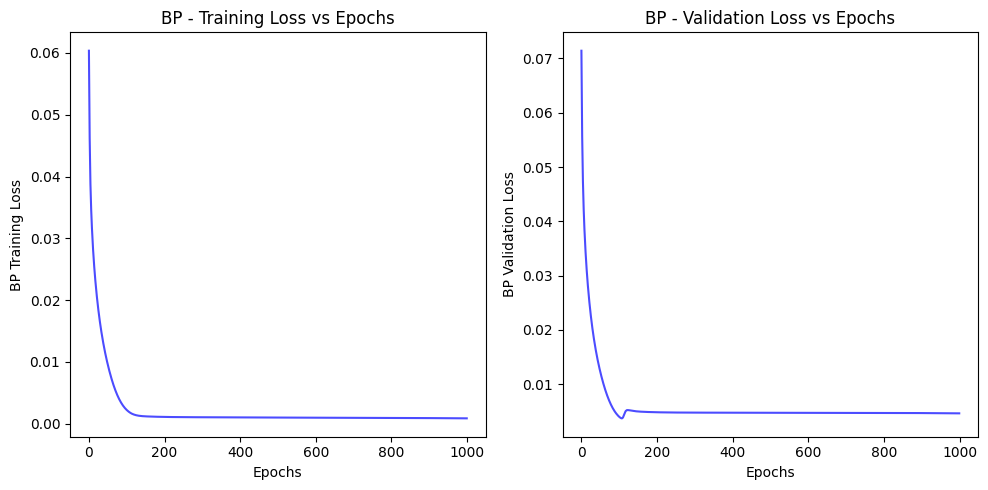
\includegraphics[width=440pt]{images/test1_error.png}
    \caption{Training error vs validation error in test index 1}
    \label{fig:image_error_test_1}
\end{figure}

\subsubsection{Test 2}

\begin{figure}[H]
    \centering
    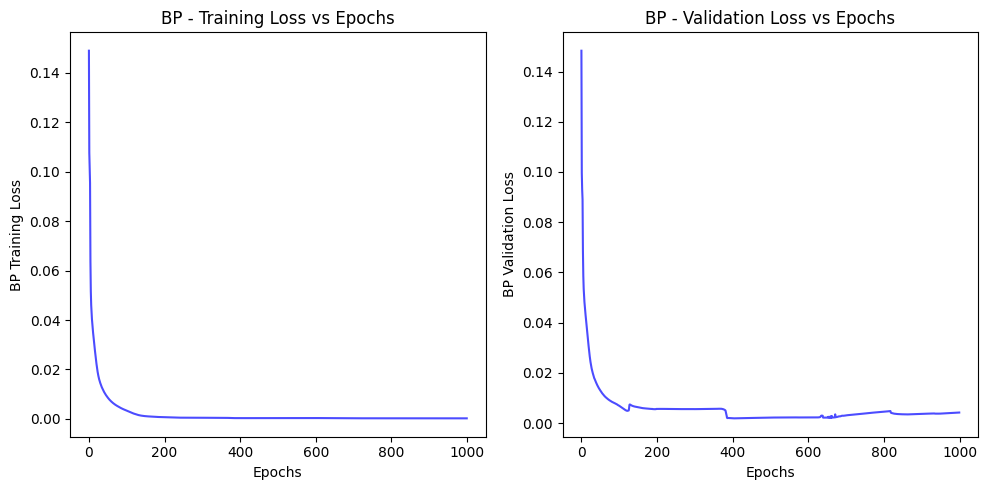
\includegraphics[width=440pt]{images/test2_error.png}
    \caption{Training error vs validation error in test index 2}
    \label{fig:image_error_test_2}
\end{figure}

\subsubsection{Test 3}

\begin{figure}[H]
    \centering
    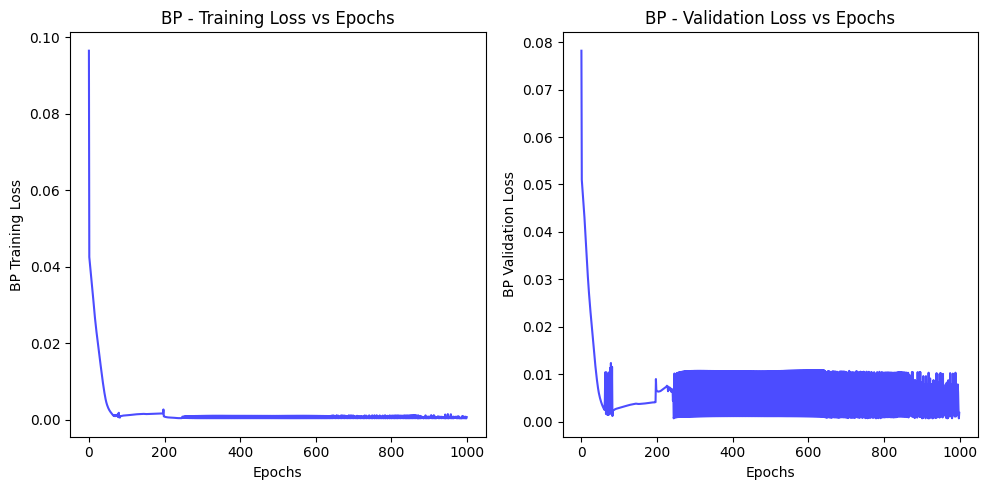
\includegraphics[width=400pt]{images/test3_error.png}
    \caption{Training error vs validation error in test index 3}
    \label{fig:image_error_test_3}
\end{figure}

\newpage

\section{Comparison with other models BP vs BP-F vs MLR-F}

When evaluating model performance, scatter plots are a useful tool. In these plots, better performance is indicated by points closer to the diagonal. 
This means the predicted values are closer to the real ones. Three new tests have been performed to compare the three models.

\vspace{1em}From the model's perspective, shows some clear trends. In Test 1, the BP-F model outperformed both BP and MLR-R models, achieving the lowest MAPE, MAE, and MSE. 
This indicates that BP-F is more accurate and reliable under these conditions.

\vspace{1em}In Test 2, BP-F again showed better performance than BP and MLR-R, with lower MAE and MSE values. However, the difference between BP and BP-F was less pronounced 
compared to Test 1. This suggests that while BP-F generally performs better, the advantage may vary depending on the specific test conditions.

\vspace{1em}Test 3 presented a different scenario where BP achieved the lowest errors, while BP-F and MLR-R had significantly higher MAPE, MAE, and MSE values. 
This indicates that BP can sometimes outperform BP-F and MLR-R, especially when the number of epochs is lower. 

\vspace{1em} In conclusion and overall, BP and BP-F models tend to perform better than MLR-R, but the choice between BP and BP-F may depend on the specific parameters 
and conditions of the test.

\subsection{Test 1}

The parameters used for the 3 models are the following ones:

\begin{table}[H]
    \centering
    \begin{tabular}{|c|c|c|c|c|c|c|}
        \hline
        \textbf{Model} & \textbf{Nº layers} & \textbf{Structure}  & \textbf{Nº epochs} & \textbf{Learning} & \textbf{Momentum} & \textbf{Activation} \\ \hline
        BP       & 3                & [16, 4, 1]    & 10000      & 0.001         & 0.001    & relu                \\ \hline
        BP-F     & 3                & [16, 4, 1]    & 10000      & 0.001         & 0.001    & relu                \\ \hline
        MLR-F    & 3                & [16, 4, 1]    & 10000      & 0.001         & 0.001    & relu              \\ \hline
    \end{tabular}
    \caption{Test 1 - Comparison between models parameters}
    \label{tab:table_parameters_comparison_1}
\end{table}

And the quality results are the following ones

\begin{table}[H]
    \centering
    \begin{tabular}{|c|c|c|c|}
        \hline
        \textbf{Model} & \textbf{MAPE}         & \textbf{MAE}         & \textbf{MSE}         \\ \hline
        BP & 8.174308e+11 & 8.011910e-2 & 6.945218e-3 \\ \hline
        BP-F & 5.832255e+11 & 5.275115e-2 & 3.506288e-3 \\ \hline
        MLR-F & 1.812658e+12 & 8.446904e-2 & 1.219164e-2 \\ \hline
    \end{tabular}
    \caption{Test 1 -Comparison between models results}
    \label{tab:table_results_comparison_1}
\end{table}

\subsubsection{Scatter plot}

\begin{figure}[H]
    \centering
    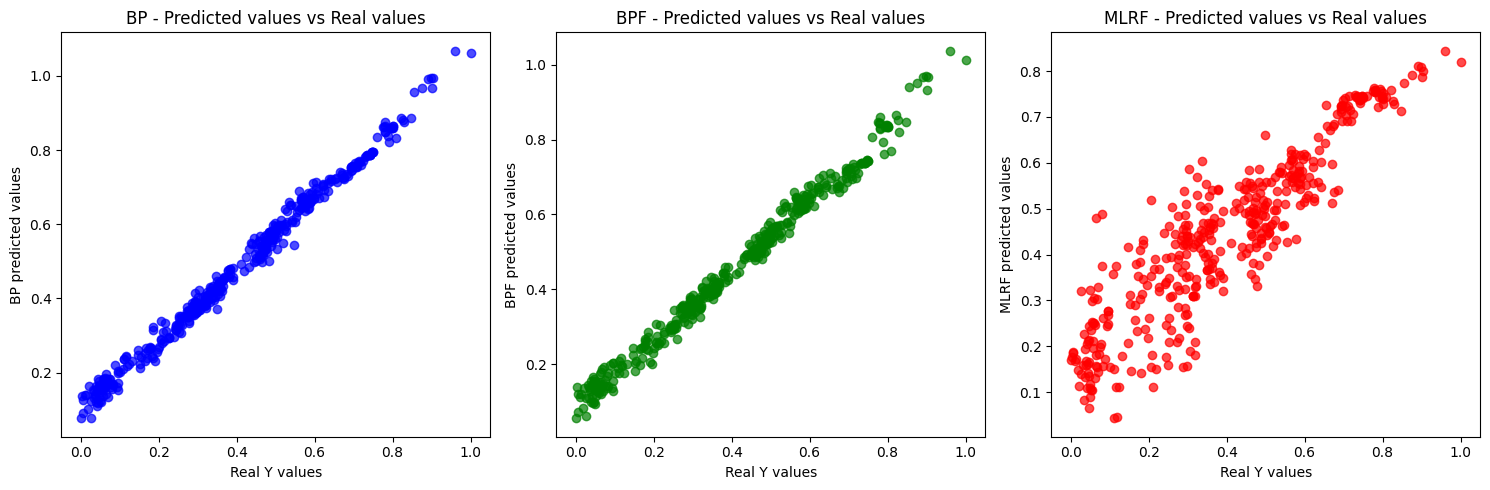
\includegraphics[width=400pt]{images/test1_scatter.png}
    \caption{Test 1 - scatter plot of the 3 models}
    \label{fig:image_scatter_comparison_1}
\end{figure}

\subsection{Test 2}

The parameters used for the 3 models are the following ones:

\begin{table}[H]
    \centering
    \begin{tabular}{|c|c|c|c|c|c|c|}
        \hline
        \textbf{Model} & \textbf{Nº layers} & \textbf{Structure}  & \textbf{Nº epochs} & \textbf{Learning} & \textbf{Momentum} & \textbf{Activation} \\ \hline
        BP       & 3                & [16, 4, 1]    & 1000      & 0.001         & 0.001    & relu                \\ \hline
        BP-F     & 3                & [16, 4, 1]    & 1000      & 0.001         & 0.001    & relu                \\ \hline
        MLR-F    & 3                & [16, 4, 1]    & 1000      & 0.001         & 0.001    & relu              \\ \hline
    \end{tabular}
    \caption{Test 2 - Comparison between models parameters}
    \label{tab:table_parameters_comparison_2}
\end{table}

And the quality results are the following ones

\begin{table}[H]
    \centering
    \begin{tabular}{|c|c|c|c|}
        \hline
        \textbf{Model} & \textbf{MAPE}         & \textbf{MAE}         & \textbf{MSE}         \\ \hline
        BP & 6.239873e+11 & 7.014470e-2 & 5.567292e-3 \\ \hline
        BP-F & 6.572347e+11 & 5.234516e-2 & 3.462514e-3 \\ \hline
        MLR-F & 1.568601e+12 & 6.542944e-2 & 7.089106e-3 \\ \hline
    \end{tabular}
    \caption{Test 2 -Comparison between models results}
    \label{tab:table_results_comparison_2}
\end{table}

\subsubsection{Scatter plot}

\begin{figure}[H]
    \centering
    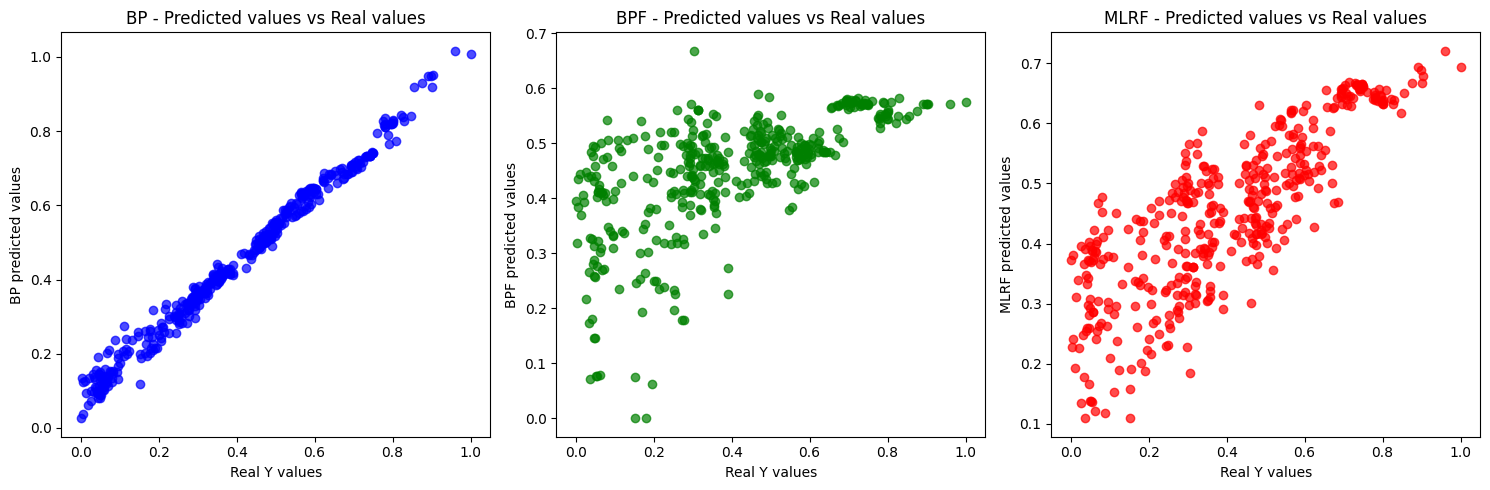
\includegraphics[width=400pt]{images/test2_scatter.png}
    \caption{Test 2 - scatter plot of the 3 models}
    \label{fig:image_scatter_comparison_2}
\end{figure}

\subsection{Test 3}

The parameters used for the 3 models are the following ones:

\begin{table}[H]
    \centering
    \begin{tabular}{|c|c|c|c|c|c|c|}
        \hline
        \textbf{Model} & \textbf{Nº layers} & \textbf{Structure}  & \textbf{Nº epochs} & \textbf{Learning} & \textbf{Momentum} & \textbf{Activation} \\ \hline
        BP       & 3                & [16, 4, 1]    & 1000      & 0.001         & 0.001    & relu                \\ \hline
        BP-F     & 3                & [16, 4, 1]    & 1000      & 0.001         & 0.001    & relu                \\ \hline
        MLR-F    & 3                & [16, 4, 1]    & 1000      & 0.001         & 0.001    & relu              \\ \hline
    \end{tabular}
    \caption{Test 3 - Comparison between models parameters}
    \label{tab:table_parameters_comparison_3}
\end{table}

And the quality results are the following ones

\begin{table}[H]
    \centering
    \begin{tabular}{|c|c|c|c|}
        \hline
        \textbf{Model} & \textbf{MAPE}         & \textbf{MAE}         & \textbf{MSE}         \\ \hline
        BP & 2.764482e+11 & 4.838344e-2 & 3.096494e-3 \\ \hline
        BP-F & 4.212754e+12 & 1.542775e-1 & 3.621248e-2 \\ \hline
        MLR-F & 3.964180e+12 & 1.188944e-1 & 2.303858e-2 \\ \hline
    \end{tabular}
    \caption{Test 3 -Comparison between models results}
    \label{tab:table_results_comparison_3}
\end{table}

\subsubsection{Scatter plot}

\begin{figure}[H]
    \centering
    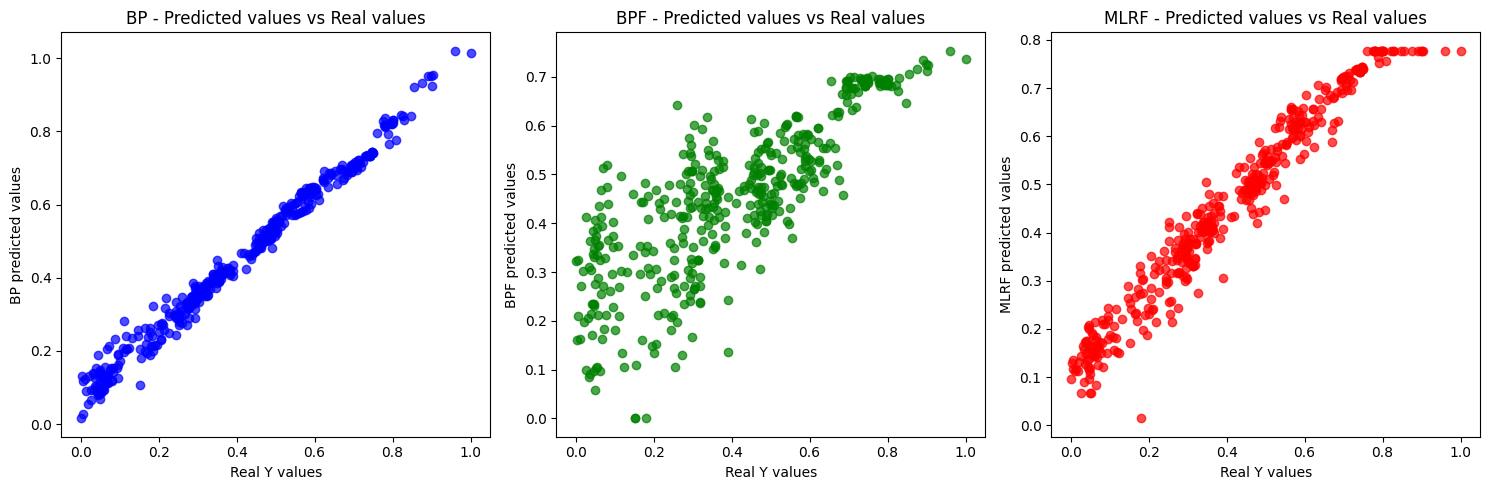
\includegraphics[width=400pt]{images/test3_scatter.png}
    \caption{Test 3 - scatter plot of the 3 models}
    \label{fig:image_scatter_comparison_3}
\end{figure}

% Please add the following required packages to your document preamble:
% \usepackage[table,xcdraw]{xcolor}
% Beamer presentation requires \usepackage{colortbl} instead of \usepackage[table,xcdraw]{xcolor}

\newpage

\begin{thebibliography}{11}

\bibitem{Gomez}
Sergio Gómez, "Supervised Learning Using Back-Propagation," Neural and Evolutionary Computation. 

\bibitem{HKP2}
Hertz, Krogh \& Palmer, Introduction to the Theory of Neural Computation, Chapter ONE: Introduction.

\bibitem{HKP}
Hertz, Krogh \& Palmer, Introduction to the Theory of Neural Computation, Chapter FIVE: Simple Perceptrons (only 5.1, 5.2, 5.4 except Convergence of Gradient Descent, 5.5), Chapter SIX: Multi-Layer Networks (all except 6.5).

\bibitem{DS}
Du \& Swamy, Neural Networks and Statistical Learning, Chapter 1: Introduction (all except 1.2.2 and 1.4).

\bibitem{LinearRegression}
Linear regression and Ordinary least squares, Wikipedia. \url{https://en.wikipedia.org/wiki/Linear_regression}

\bibitem{LogisticRegression}
Logistic regression, Wikipedia. \url{https://en.wikipedia.org/wiki/Logistic_regression}

\bibitem{NaiveBayes}
Naive Bayes classifier, Wikipedia. \url{https://en.wikipedia.org/wiki/Naive_Bayes_classifier}

\bibitem{KNN}
K-Nearest Neighbors, Wikipedia. \url{https://en.wikipedia.org/wiki/K-nearest_neighbors_algorithm}

\bibitem{Kotsiantis2006}
S. B. Kotsiantis, D. Kanellopoulos, and P. E. Pintelas, "Data Preprocessing for Supervised Learning," International Journal of Computer Science, vol. 1, no. 2, 2006, ISSN 1306-4428.

% \bibitem{IEEENTRU}
% IEEEP1363, Standard Specifications For Public-Key Cryptography. 
% \url{http://grouper.ieee.org/groups/1363/}.

% \bibitem{Smart2023}
% Nigel Smart, "Cryptography: An Introduction (3rd Edition)," 2023.

% \bibitem{Banoth2023}
% Rajkumar Banoth and Rekha Regar, "An Introduction to Classical and Modern Cryptography," 2023.
% \url{https://link.springer.com/chapter/10.1007/978-3-031-32959-3_1}

% \bibitem{Richter2022}
% Maximilian Richter et al., "A Mathematical Perspective on Post-Quantum Cryptography," 2022.
% \url{https://www.mdpi.com/2227-7390/10/15/2579}

% \bibitem{Ishai2019}
% Yuval Ishai et al., "Advances in Cryptology EUROCRYPT 2019," 2019.
% \url{https://link.springer.com/book/10.1007/978-3-031-68394-7}

% \bibitem{Koshiba2007}
% Takeshi Koshiba, "Security Notions for Quantum Public-Key Cryptography" 2007.
% \url{https://arxiv.org/abs/quant-ph/0702183}

\end{thebibliography}

\end{document}
